\chapter{Specific requirements}

\section{External Interface Requirements }
The system to be developed has to store information about cars, accounts, all data related to accounting and administration sectors and also data produced by system itself to manage the rental service. The external services called by the system directly interact with it.
External Interface Required for PowerEnjoy:
\begin{itemize}
\item A database;
\item A SMS gateway.
\item A Push Service;
\end{itemize}

\subsection{User interfaces}
\subsubsection{Home mobile app}
\begin{center}
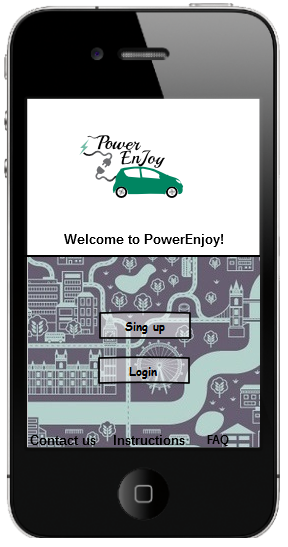
\includegraphics[]{../images/mookup/Homepage_mobile}
\end{center}

\clearpage
\subsubsection{Home web app}
\begin{center}
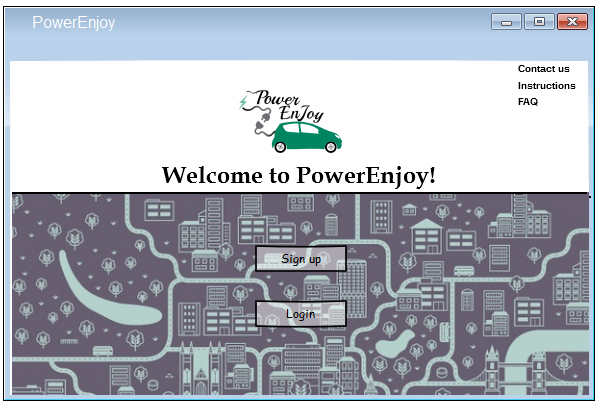
\includegraphics[]{../images/mookup/homepage_web}
\end{center}

\clearpage
\subsubsection{Reservation mobile app}
\begin{center}
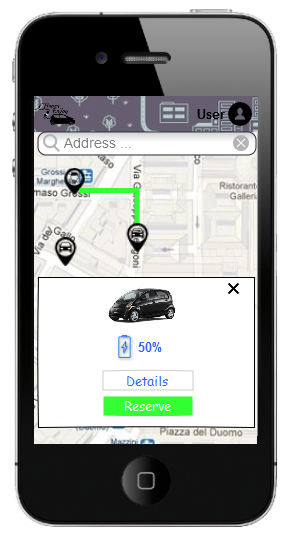
\includegraphics[]{../images/mookup/Reservation_mobile}
\end{center}

\clearpage
\subsubsection{Reservation web app}
\begin{center}
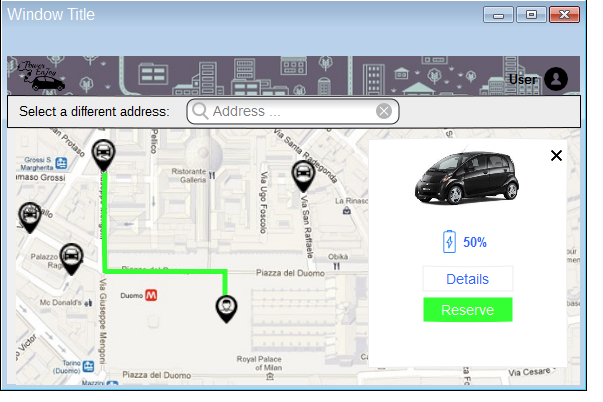
\includegraphics[]{../images/mookup/Reservation_web}
\end{center}

\clearpage
\subsubsection{Account details mobile app}
\begin{center}
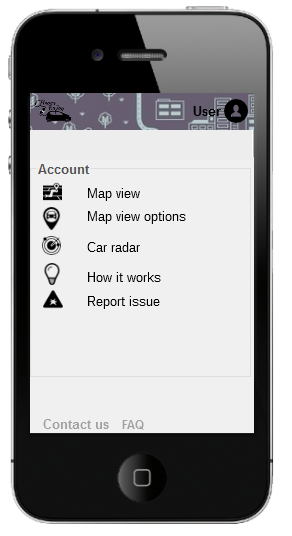
\includegraphics[]{../images/mookup/Account_mobile_sx}

\clearpage
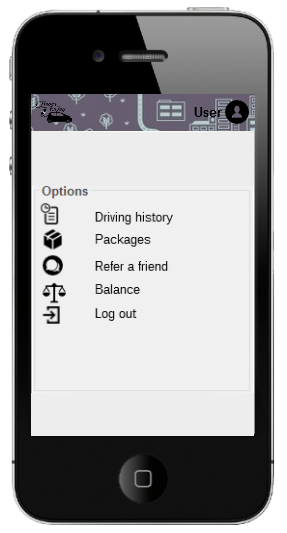
\includegraphics[]{../images/mookup/Account_mobile_dx}
\end{center}

\clearpage
\subsubsection{Account details web app}
\begin{center}
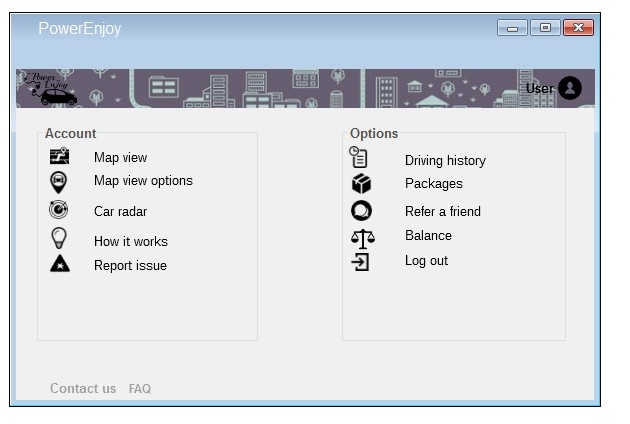
\includegraphics[]{../images/mookup/Account_web}
\end{center}




\subsection{Hardware interfaces}
The hardware interfaces of our system are:
\begin{itemize}
\item Owned by the clients: a computer or a mobile device in order to complete all the actions concerning registration, login, reservation procedure and also to manage his/her account data.
\item Owned by PowerEnJoy: a GPS navigation device for each car, that represents the main interface between the client and the system during the ride period.
Its main functionalities are:
\begin{enumerate}
\item Require the client his/her personal pin code;
\item Let the client choose all the options related to his/her ride;
\item Show the driver all the notifications sent by the system;
\item Let the client choose to end his/her rent.
\end{enumerate}
\end{itemize}
\subsection{Software interfaces}
\begin{itemize}
\item DBMS: MySQL
\item Proxy server: Nginx
\item Application server: Express.js
\item Web app UI library: Riot.js
\item Websocket library: Socket.io
\end{itemize}
\subsection{Comunication interfaces}
The system communicates using websocket, that makes possible to have an effective real-time application.

\section{Functional requirements}

\subsection{[G1] - The Registered Client can hire a car through web/mobile application}
\begin{enumerate}[label=\textbf{R1.\arabic*)}]
\item The system allows the Registered Client to choose the car to hire only between the available ones.
\item The system allows only one reservation per time for each Registered Client.
\item The system allows the Registered Client to cancel his/her request.
\item The system considers the reservation request as valid for at most one hour from the moment in which the request of hiring is accepted.
If the Registered Clients doesn’t reach the car before this time expires, the system gives him/her a penalty of one euro and mark the car as ‘available’ again.
\item When a car is reserved the system marks it as ‘unavailable’.
\item The system unlock the chosen car only when the Registered Client is nearby and he/she communicates this to the system through the application.
\item The system locks the car when the Registered Client parks it in a safe area or in a power grid station and he/she communicates the system the intention of ending the rent.
\item When the rent is finished the system marks the car as “available” again.
\item The system starts charging the Registered Client for a given amount of money per minute as soon as the engine ignites.
\item The system stops charging the user as soon as the car is parked in a safe area or in a power grid station and the Registered Client exits the car.
Then the system starts the payment procedure.
\item The system allows the Registered Client to start driving if and only if he/she insert his/her personal code.
\item The system allows the Registered Client to choose an address in which he/she wants to hire a car or if he/she wants to be located through the GPS signal.
\item The system must supervise the charge of the car during all the rental period, showing the current charge on the GPS navigation device.
It also has to show a warning notice if the charge is equal to the minimum possible charge admitted.
\item The system allows the Registered Client to find the location of an available car within a certain distance from his/her current location.
\end{enumerate}

\subsection{[G2] - The Registered Client can hire a car through an SMS.}
\begin{enumerate}[label=\textbf{R2.\arabic*)}]
\item The system must check that the SMS is sent from a phone number related to a Registered Client account.
\item The system accepts only well formed SMS messages, that follow a precise pattern: “Action + plate”.
\item The system must check a correspondence of the plate indicated by the Registered Client with one of the cars in its database labeled as available.
\item The system sends an SMS to communicate the Registered Client the outcome of his/her request.
\item If the request has been accepted, the system marks the car as ‘unavailable’ and reserves it.
\item The system unlocks the car if and only if it receives an ‘unlock’ SMS from  the same phone number that has reserved it.
\item The system deletes the request of reservation if and only if it receives a ‘delete’ SMS from the same phone number that has done the reservation. The system and mark the car as available again.
\item The system considers the reservation request as valid for at most one hour from the moment in which the request of hiring is accepted. If the Registered Client doesn’t send an ‘unlock’ SMS before this time expires, the system gives him/her a penalty of one euro and mark the car as ‘available’ again.
\item When the rent finishes the system sends the Registered Client an SMS with a recap of the overall cost of the rent.
\item The system locks the car when the Registered Client parks it in a safe area or in a power grid station and he/she communicates the system the intention of ending the rent.
\item The system marks the car ‘available’ again once it is locked.
\item The system allows the Registered Client to start driving if and only if he/she insert his/her personal code.
\item The system starts charging the Registered Client for a given amount of money per minute as soon as the engine ignites.
\item The system stops charging the user as soon as the car is parked in a safe area or in a power grid station and the Registered Client exits the car. Then the system start the payment procedure.
\item The system must supervise the charge of the car during all the rental period, showing the current charge on the GPS navigation device. It also has to show a warning notice if the charge is equal to the minimum possible charge admitted.
\end{enumerate}

\subsection{[G3] - The Guest Client can register himself/herself into the system as Registered Client.}
\begin{enumerate}[label=\textbf{R3.\arabic*)}]
\item The system requests an e-mail and a telephone number during the registration.
\item The system rejects an e-mail and a telephone number already used by another Registered Client.
\item Once the registration procedure is successfully completed, the system sends a confirmation email to the new Registered Client.
\item The system checks if e-mails or telephone numbers are well formed.
\item The system considers a user as a Registered Client if and only if he/she opens the activation link in the confirmation e-mail.
\item The system considers a phone number valid if and only if the user inserts the code sent by the system through an SMS.
\item The registration procedure requires the Guest Client to indicate his/her driving licence.
\item The system requires the Registered Client to specify one valid payment method.
\item The system must send back to the Registered Client’s email a password that he/she can use to access the system.
\end{enumerate}

\subsection{[G4] - Registered Clients can login into the system.}
\begin{enumerate}[label=\textbf{R4.\arabic*)}]
\item The system allows only Registered Clients, with valid access credentials to login in the application.
\item The system allows Registered Clients that have forgotten their password to recover it, sending an email with a temporary password to the e-mail address indicated during the registration procedure.
\item The system requires Registered Clients to enter valid username (email address) and password to login.
\end{enumerate}

\subsection{[G5] - The Logged Client can manage his/her sensible data.}
\begin{enumerate}[label=\textbf{R5.\arabic*)}]
\item The system allows the Logged Client to change his/her payment method.
\item The system allows the Logged Client to change his/her current password.
\item The system allows Logged Client to change his/her own email address. The system considers valid the new email address if and only if the Logged Client open the activation link in the confirmation e-mail sent by the system at the end of the procedure.
\item The system allows Logged Client to change his/her phone number. The activation of the new phone number is completed only when the Logged Client insert the code sent by the system through an SMS to the new phone number.
\item The Registered Client can manage his/her requests of hiring.
\item The system allows Registered Client to cancel his/her request of hiring a car.
\item The system allows Registered Client, once logged into the system, to display his/her history of hiring request.
\end{enumerate}

\subsection{[G6] - Ensure the Registered Client the possibility to receive a discount on his/her last ride.}
\begin{enumerate}[label=\textbf{R6.\arabic*)}]
\item During the entire rent period the system must check if some conditions happen in order to apply a discount on the final rent cost are satisfied.
\item The system allows the Registered Client to enable the ‘save money’ option at the beginning of his/her ride through the GPS navigation device.
\item If the system detects the Registered Client took at least two other passengers onto the car, the system applies a discount of 10\% on the last ride.
\item If a car is left with more than 50\% of charge, the system applies a discount of 20% on the last ride.
\item If a car is left in a power grid station and the Registered Client takes care of plugging the car into the power grid, the system applies a discount of 30\% on the last ride.

\end{enumerate}

\subsection{[G7] - Ensure a uniform distribution of cars in the city.}
\begin{enumerate}[label=\textbf{R7.\arabic*)}]
\item The system, considering the actual distribution of the cars in the area, must always highlight through the GPS navigation device the area in which the client may park the car
\end{enumerate}

\subsection{[G8] - Guarantee to have always a minimum number of cars in the system with enough charge to be hired.}
\begin{enumerate}[label=\textbf{R8.\arabic*)}]
\item The system must report a warning if it detects that the number of cars in the system with enough charge to be hires is less than the minimum possible.
\end{enumerate}

\subsection{[G9] - Allow the system administrator to update and check data in the database of the system.}
\begin{enumerate}[label=\textbf{R9.\arabic*)}]
\item The system must disallow not certified system administrators to perform such operations.
\item The system must guarantee integrity and consistency of data after eventual updates performed on them.
\item The system allows the system administrators to add new Safe Area in the set of Safe Area predefined by the management system.
\end{enumerate}

\subsection{[G10] - Guarantee a correct interoperability of the system with external services.}
\begin{enumerate}[label=\textbf{R10.\arabic*)}]
\item The system must always be able to perform requests to external services, when they’re needed.
\end{enumerate}

\subsection{[G11] - Ensure that a Registered Client’s bad behaviour is punished with the application of some penalties.}
\begin{enumerate}[label=\textbf{R11.\arabic*)}]
\item If a car is left at more than 3 KM from the nearest power grid station, the system charges 30\% more on the last ride.
\item If a car is left with more than 80\% of the battery empty, the system charges 30\% more on the last ride.
\end{enumerate}
\section{Scenario}
\subsection{Scenario 1}
Frank and his flatmates have nothing to eat for lunch and they need to go to the supermarket, that is not close to Frank’s house.
The thought to do the same long road two times is not an awesome picture in guys’ minds.
Fortunately yesterday Frank saw an advertisement about the car sharing service of PowerEnJoy, so he downloads the mobile application and registers himself to use that service.
Frank activates the GPS signal tracking to let the app locates his position and the app shows him a car near his house.
So they make a reservation and exit from home to reach the car.
Once arrived, Frank open again the app to communicate to PowerEnJoy he’s nearby: the system unlocks the doors and Frank and his friends are able to jump in.
The car starts the engine only after the insertion of the personal account PIN, provided during the registration: Frank enters it and the car becomes able to be turned on.
After reaching the supermarket, Frank and his friends don’t want to leave the reservation of the car, because they know there is the possibility to find no cars nearby later: so they decide to leave the rent in “Pit Stop” mode.
After the shopping they come back home, reactivating the “Go” mode.
While driving Frank sees in the screen of the GPS navigation device the evaluation of the amount of money he is going to pay.
So he decides to choose the option save money to obtain a discount: he inserts the address of his house and the system indicates him where to leave the car in order to have a discount.
So he reaches the station and leaves the car in a specific space, where is also possible to plug the car to the power grid.
He terminates his rent choosing the option on the GPS navigation device  “To the Box”.
After that he has 30 seconds to plug the car to the power grid, to achieve the discount on that ride.

\subsection{Scenario 2}
Mrs. Hilly is a dynamic old lady.
Her grandson talked to her about PowerEnJoy and its innovative system to share cars in an ecological way with a cheap fare.
This service seems suitable for Hilly because she doesn’t have an internet connection but is really skilled to use SMS, the first way to communicate with her friends.
So her nephew helps her to complete the registration.
Hilly today has a medical examination and the hospital is too far to reach only with her legs: so she starts walking on the road, hopeful to find a PowerEnJoy car to rent.
After few meters, she gets close to a PowerEnJoy car and starts to follow the instructions given by her grandson: she enters the number of the service as addressee and as text the caption “Rent” followed by the plate of the car.
After few seconds she receives an SMS that confirms her reservation.
So she sends another SMS with the caption “Open” and waits until the doors of the car are unlocked by the system.
Then she enters her personal code through the GPS navigation device and drives to the hospital.

\subsection{Scenario 3}
Last week Jhonny bought a train ticket to come back home.
It’s 14:25 and the departure time is fixed at 15:00: Jhonny is late and he thinks the best way to arrive in time at the train station is to rent a car of PowerEnJoy.
Fortunately there’s one near him, so he opens the mobile application and reserves it.
Once entered in the car and arrived at the station, he realizes there’s no park available near it and the only way to leave it is to be double-parked.
So he leaves the car and takes his train. After a short time, some traffic officers sees the car in double-park: so they jump out the car and fine a ticket.
Meanwhile Lucy is arriving at destination (the same train station) and she has a heavy handbag to bring at home, so decides to hire a PowerEnJoy.
She arrives at the car and immediately sees the ticket on the windscreen of the car.
To avoid all possible problems Lucy, before starting her ride, inserts in the GPS navigation device the presence of a ticket and then starts her trip to home.

\subsection{Scenario 4}
Milan has to face a big problem constantly present in daily life: pollution.
For this reason the administrative offices of the city have decided to announce the alternation of cars traffic, basing it on the numbers of the plates of the cars.
Today there’s the opportunity to travel only for the owners of cars having an even plate number.
Unfortunately Shaun owns only a car with odd plate number, so he can’t use his car.
A lot people have found a solution taking the public transports but Shaun can’t do that, because he has to go in a zone of the city unreachable by them.
Thus he thinks it’s a perfect situation to try PowerEnjoy service.
He opens the mobile application and, as he also presumed, the nearest car is about 3 kilometers far from him, but he has an important appointment and he can’t be late for that.
So he starts walking to the car, following the instructions given by the app that estimates 40 minutes to reach the position of the car.
It’s been 30 minutes when Shaun is about 2.3 kilometers far from the car and the app shows him a warning reciting “Ehy Shaun, you have 30 minutes to reach the car.
After that lapse of time your request won’t be considered still valid and you will have to pay a fee of 1 EUR”.
Shaun doesn’t care about the message because he knows he is nearby.
Once arrived, he sends the request to open the doors of the car and jump in.

\subsection{Scenario 5}
Sandy wants to go to a concert not so far from her house but she doesn’t want to arrive walking, because of the low security of the road that she has to pass through.
The doors to enter in the concert field are going to be opened soon and she wants to hire a PowerEnJoy car: she opens her computer browser and goes on www.powerenjoy.it and inserts the address of her house and chooses a car among the available ones.
Sandy is a fan of PowerEnJoy and she wants to see the history of her previous requests.
Thus open the profile page and click on History: the site shows her all the requests advanced in the past and also the last one.
It’s late and Sandy has to go, so starts moving to reach car.
Once exited the house, it starts raining: unfortunately the concert is hold in an open space and if she go, she will get sick.
So she decides to come back home and cancel the request through the History panel of the site.

\subsection{Scenario 6}
After a birthday party, Paul has to come back home but it’s too late so there aren’t public transportations anymore.
Paul wants to hire a car with PowerEnJoy but he is worried about how much he is going to pay.
So he decides to take advantage of all the possibility to obtain a discount, since he already used PowerEnJoy a lot of times.
First of all he finds three friends, that lives near him, to join him in the car.
So they hire a car, Paul inserts the destination address in order to choose the option “save money”.
As soon as the engine ignites the sensors of the system situated in the car detect that there are three more people with the driver, so it will apply another discount to the final total amount.
When they arrive at the destination, Paul is happy because he has arrived home in a brief time paying a little amount of money.

\subsection{Scenario 7}
James usually goes to work walking.
Since the day is rainy he decides to hire a car of PowerEnjoy.
When he finally enters the car, he finds out that the car has been left in bad conditions by the previous user.
So before starting his ride, James reports the system all the present issues of the cars through the GPS navigation device, in order to not be responsible of them and to help PowerEnjoy to take measures.
Then James reaches his destination without problems.

\clearpage
\section{UML models}

\subsection{Use cases diagram}
\subsubsection{General use case}
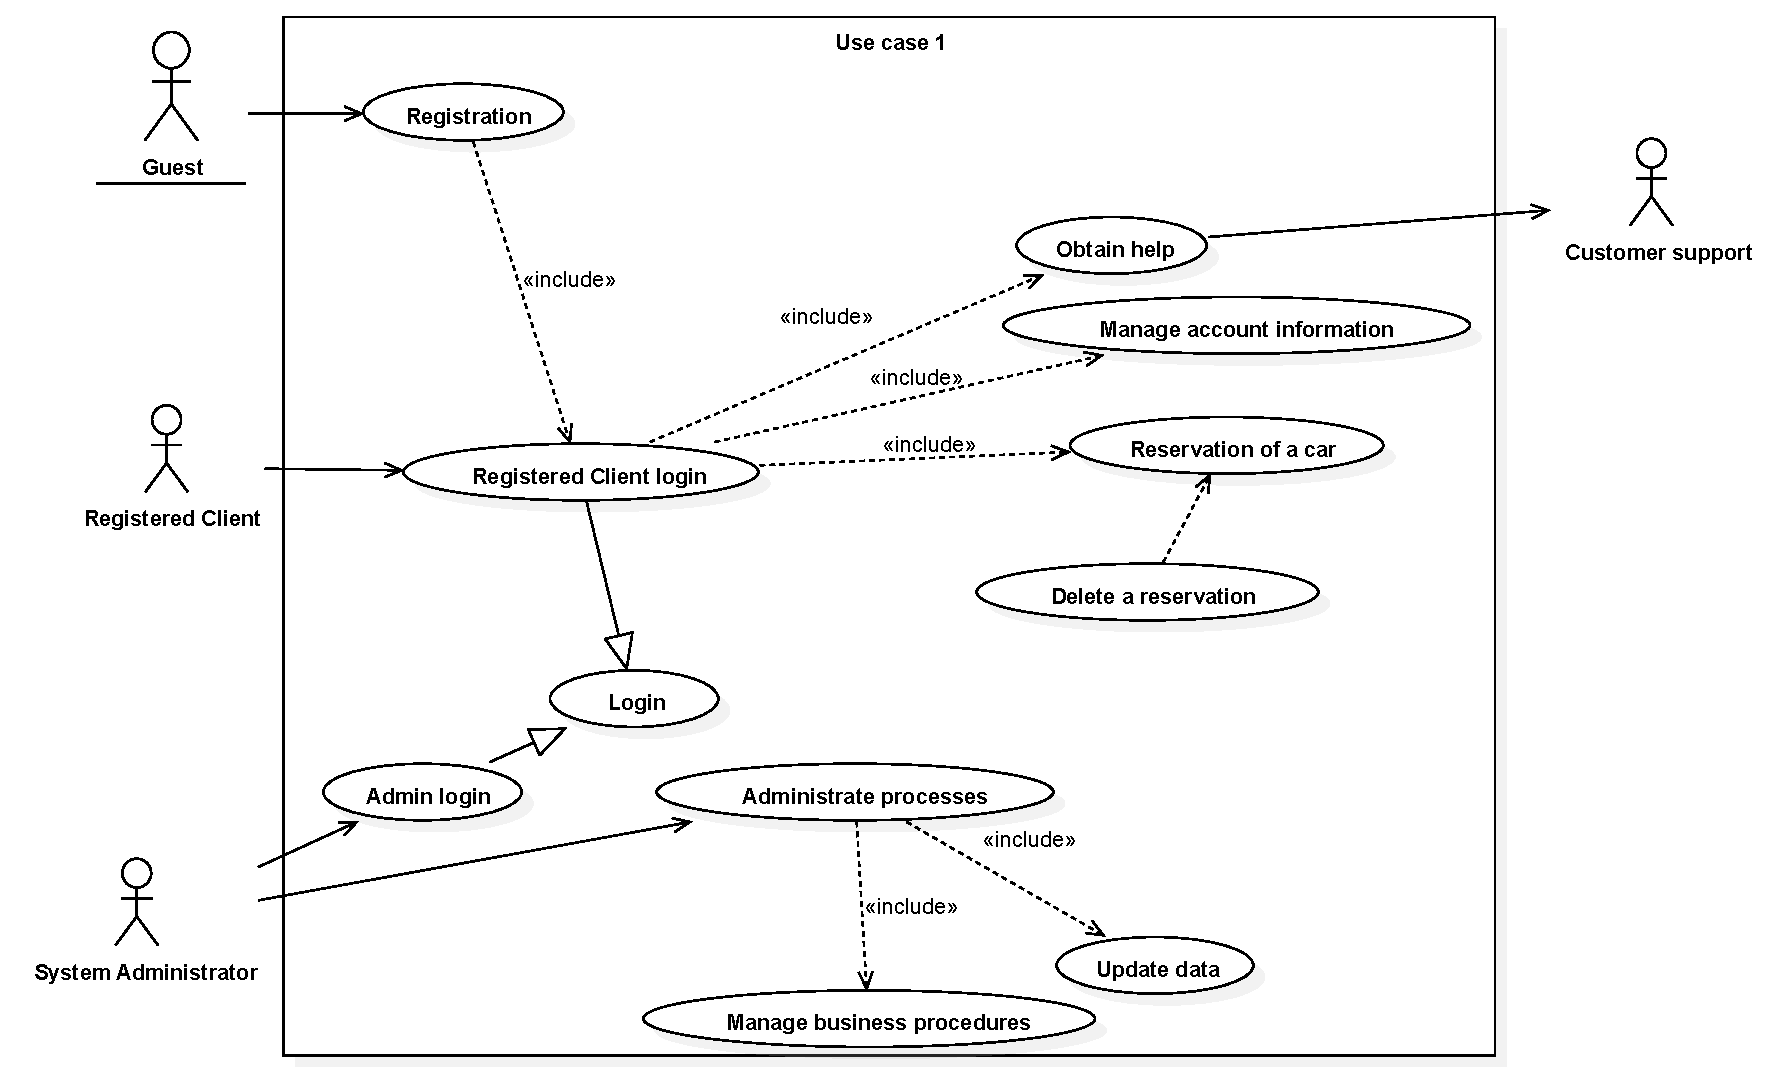
\includegraphics[width=\textwidth, keepaspectratio]{../images/diagram/use_cases/general.pdf}

\subsubsection{Rent use case}
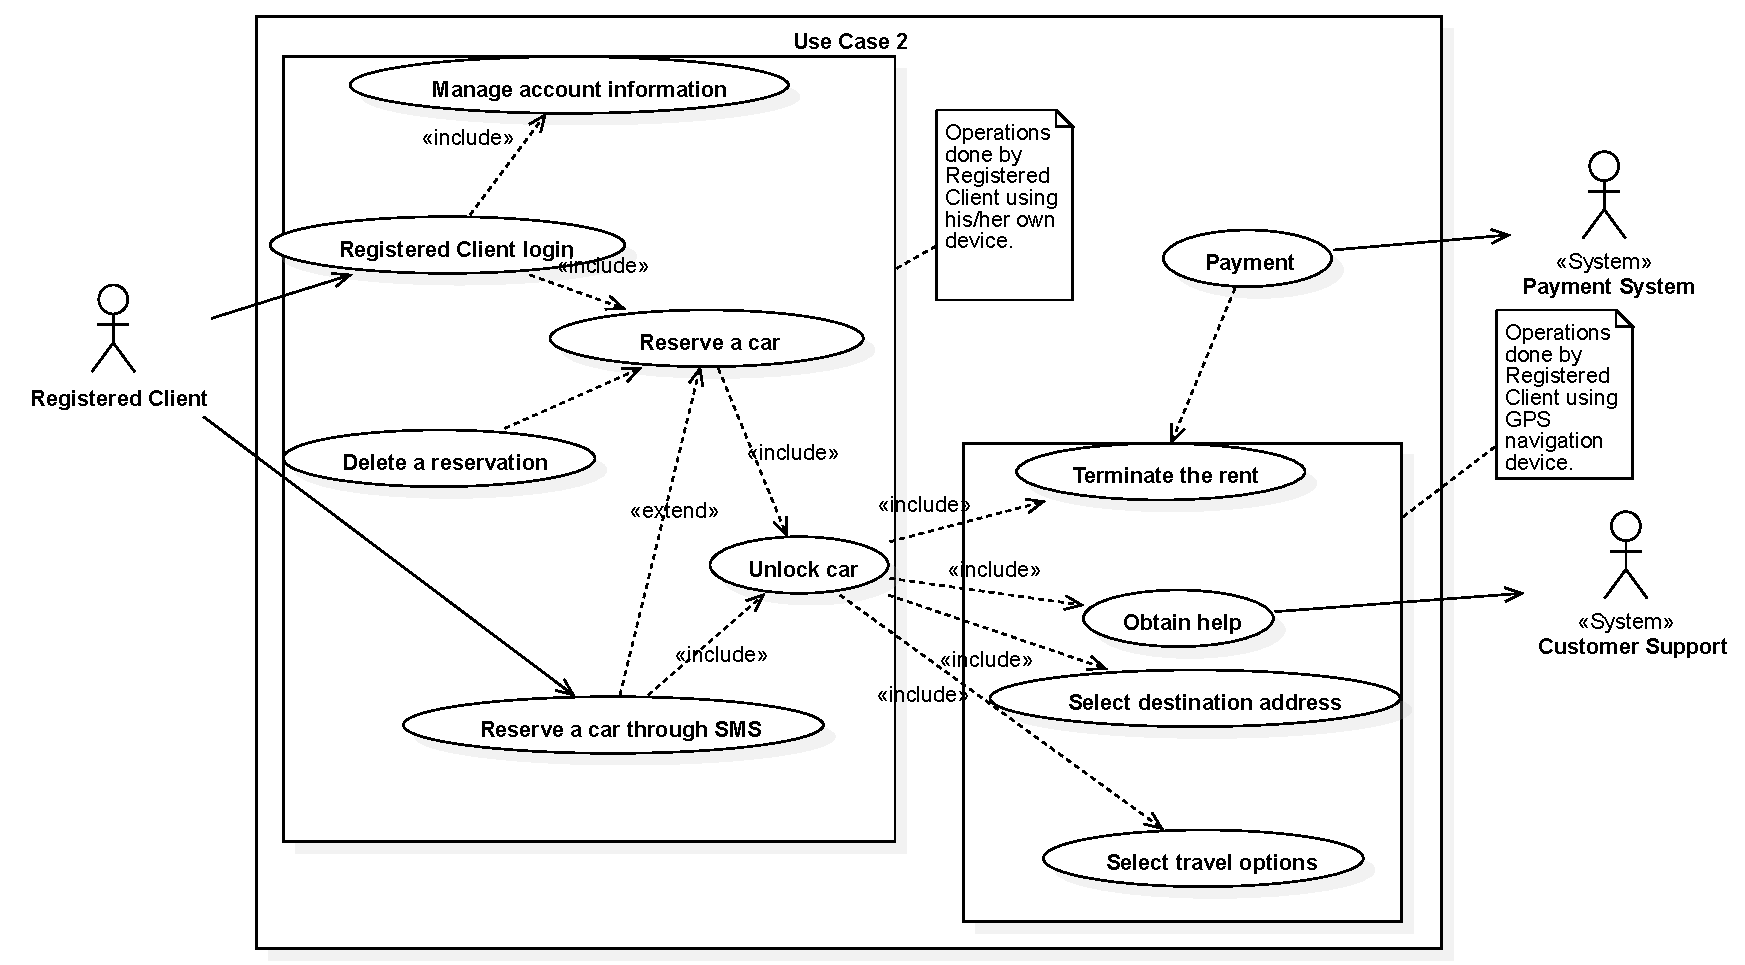
\includegraphics[width=\textwidth, keepaspectratio]{../images/diagram/use_cases/rent.pdf}

\clearpage
\subsection{Use cases description}
\subsubsection{Registration}

\begin{table}[!h]
\begin{tabularx}{\linewidth}{l|X}
\centering
Name & Sign up \\ \hline
Actor & Guest \\ \hline
Entry conditions & -- \\ \hline
Flow of events & 1. Guest clicks the "Sign up " button and the registration page is shown. \\
& 2. He/she fills the form with his/her personal details and presses the “Sign Up” button.\\
& 3. The system checks the data submitted by the guest, in particular if all the mandatory fields have been filled, and if there are no problems he/she is registered into the system. In addition the system sends back to the new user an email with an activation link and a password that he/she can use to access the system.\\
& 4. The user opens the email and clicks the activation links. The system activates the user. \\ \hline
Exit conditions & The user receives an email to confirm the registration and a password to login \\ \hline
Exceptions & If one value of the form is not valid or missing(concerning the mandatory fields), the registration is not possible and the app shows an alert indicating the errors. If the user is already registered with the information provided, the system forbid him/her to create a new account. \\
\end{tabularx}
\end{table}

\clearpage

\subsubsection{Login}

\begin{table}[!h]
\begin{tabularx}{\linewidth}{l|X}
\centering
Name & Sign in \\ \hline
Actor & Guest, Registered client \\ \hline
Entry conditions & Guest must already have credentials \\ \hline
Flow of events & 1. Guest clicks “Sign in” button and the login page is shown. \\
& 2. He/she writes his/her username and password and clicks the “Sign in” button.\\
& 3. The system checks the credentials and if they are valid the user is logged. \\
& 4. The systems shows the main page to the user. \\ \hline
Exit conditions & Guest is promoted to a Registered client. \\ \hline
Exceptions & If the credentials passed to the system are not valid the app shows an alert indicating the errors. If the Registered Client doesn’t remember either his/her username or his/her password the system allows to start the procedure to recover it. \\
\end{tabularx}
\end{table}

\clearpage
\subsubsection{Reservation through web/mobile application}
\begin{table}[!h]
\begin{tabularx}{\linewidth}{l|X}
\centering
Name & Reserve a car through web/mobile application \\ \hline
Actor & Registered client \\ \hline
Entry conditions & Registered Client must be already logged into the system. \\ \hline
Flow of events & 1. The Registered Client look for a car nearby his/her current position or near a specified address. \\
& 2. The Registered Client makes a reservation of a car, by a click on the “Reserve” button.\\
& 3. The Registered Client reaches the reserved car and clicks on the “I’m nearby” button, to let the system unlock the car doors. \\
& 4. The Registered Client enters the car and insert in the GPS navigation device his/her personal pin code. \\ \hline
Exit conditions & The Registered Client terminates his/her rent through the “Terminate Rent” button in the GPS navigation device and automatically pays for the rent through the payment method specified during the registration procedure. \\ \hline
Exceptions & If the Registered Client doesn’t reach the reserved car in one hour from the reservation the system applies him/her a penalty, marks the reservation as not valid anymore and the car as available again. If the Registered Client has already an active reservation, the system shows an alert indicating the kind of error. \\
\end{tabularx}
\end{table}

\clearpage
\subsubsection{Reservation through SMS}
\begin{table}[!h]
\begin{tabularx}{\linewidth}{l|X}
\centering
Name & Reserve a car through SMS \\ \hline
Actor & Registered client \\ \hline
Entry conditions & The Registered Client is nearby the car he/she wants to rent. \\ \hline
Flow of events & 1. The Registered Client sends an SMS with the caption “Hire” followed by the plate of the car he/she wants to rent. \\
& 2. The Registered Client receives a confirmation SMS and writes another SMS with the caption “Open”.\\
& 3. The Registered Client waits until the doors are unlocked. \\
& 4. The Registered Client enters the car and insert in the GPS navigation device his/her personal pin code. \\ \hline
Exit conditions & The Registered Client terminates his/her rent through the “Terminate Rent” button in the GPS navigation device and automatically pays for the rent through the payment method specified during the registration procedure. \\ \hline
Exceptions & If the Registered Client doesn’t send the “Open” SMS within one hour  the system applies him/her a penalty, marks the reservation as not valid anymore and the car as available again. If the phone number used for reservation is not associated to any Registered Client in the database, the system sends a warning SMS pointing out the error. If the phone number is associated to a Registered Client but he/she has already an active reservation, the system sends a warning SMS pointing out the error. \\
\end{tabularx}
\end{table}

\clearpage
\subsubsection{System Administrator login}
\begin{table}[!h]
\begin{tabularx}{\linewidth}{l|X}
\centering
Name & System Administrator login \\ \hline
Actor & System Administrator \\ \hline
Entry conditions & The system administrator is registered in the system\\ \hline
Flow of events & 1. The system administrator opens the administration page. \\
& 2. The system administrator inserts his/her credentials.\\ \hline
Exit conditions & The system administrator is now capable of doing his/her tasks. \\ \hline
Exceptions & If the credentials provided are not valid, the system shows an alert indicating the error. \\
\end{tabularx}
\end{table}

\subsection{Sequence diagrams}

\subsubsection{Login}
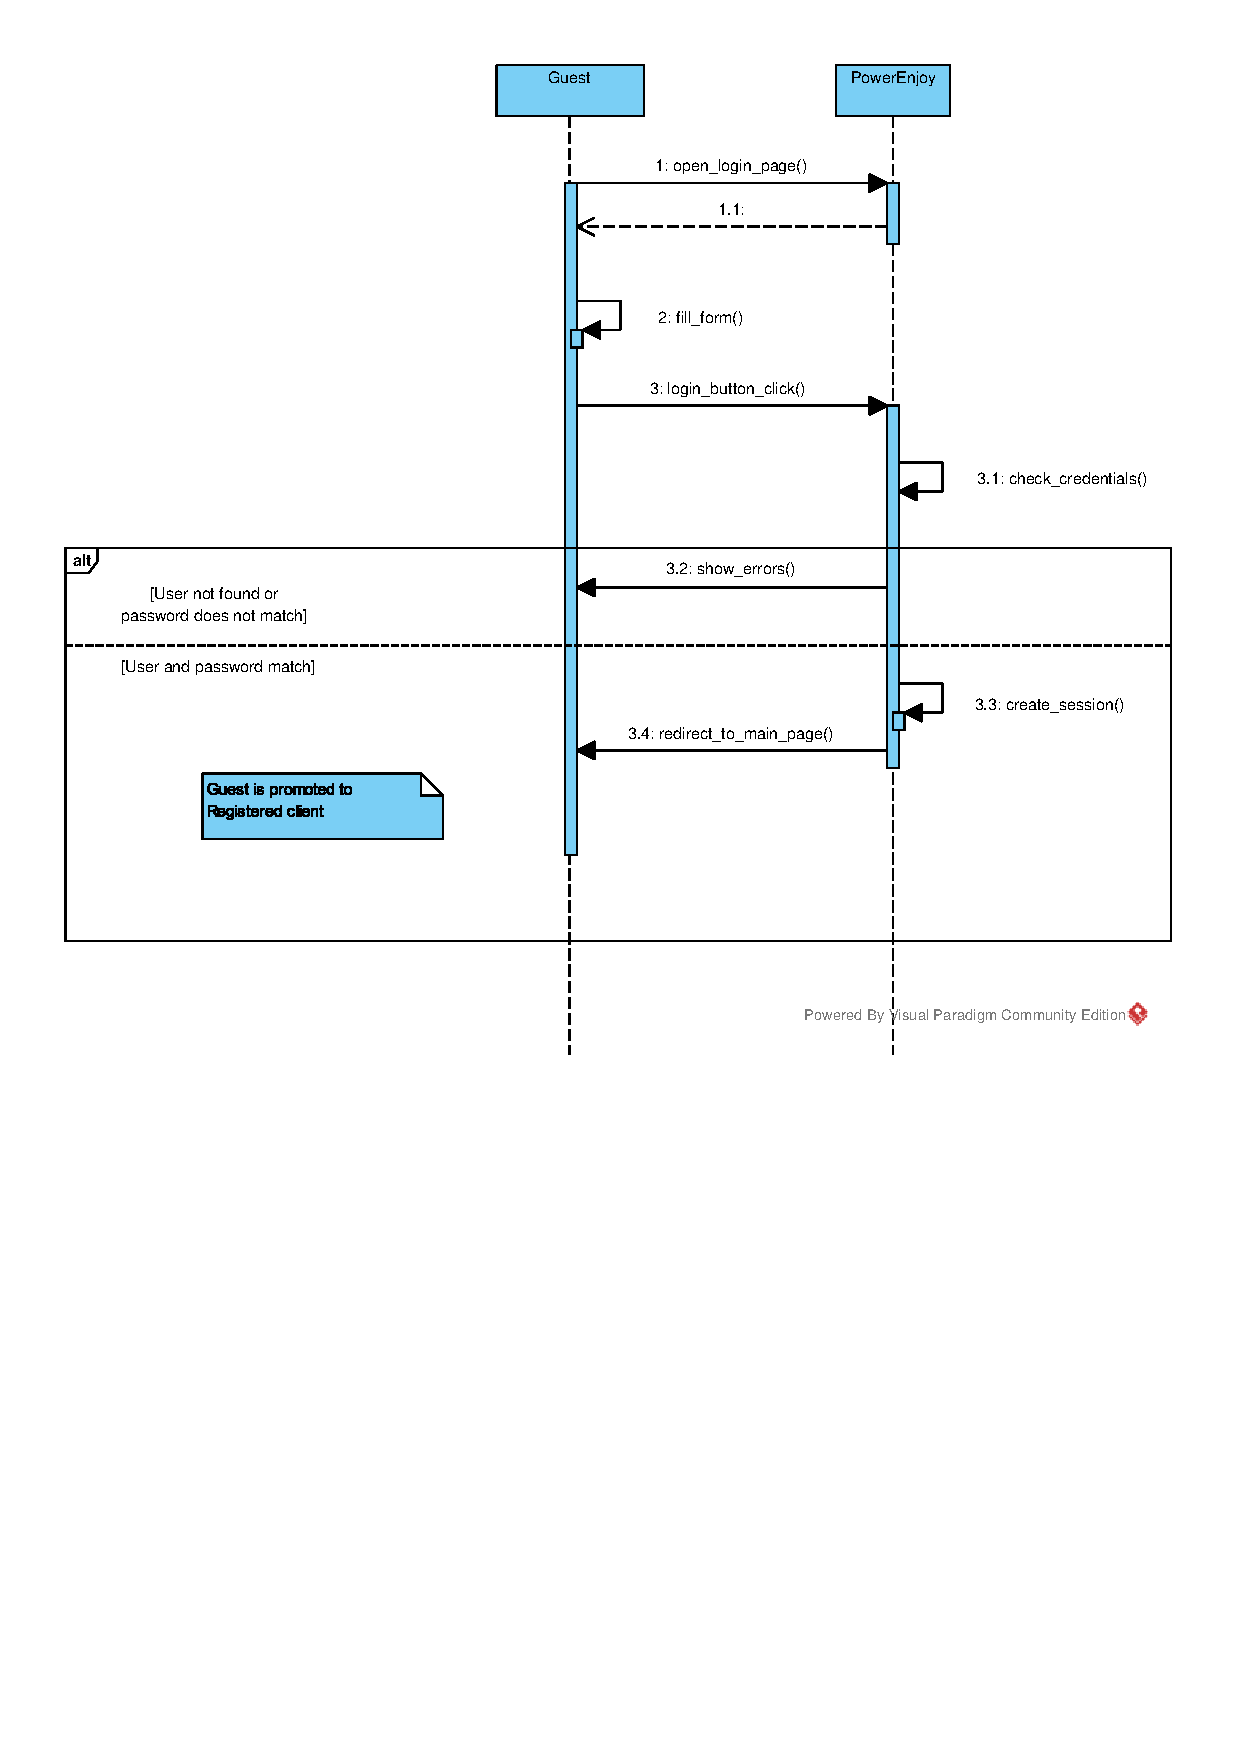
\includegraphics[width=\textwidth, keepaspectratio]{../images/diagram/sequence/login.pdf}


 \subsubsection{Registration}
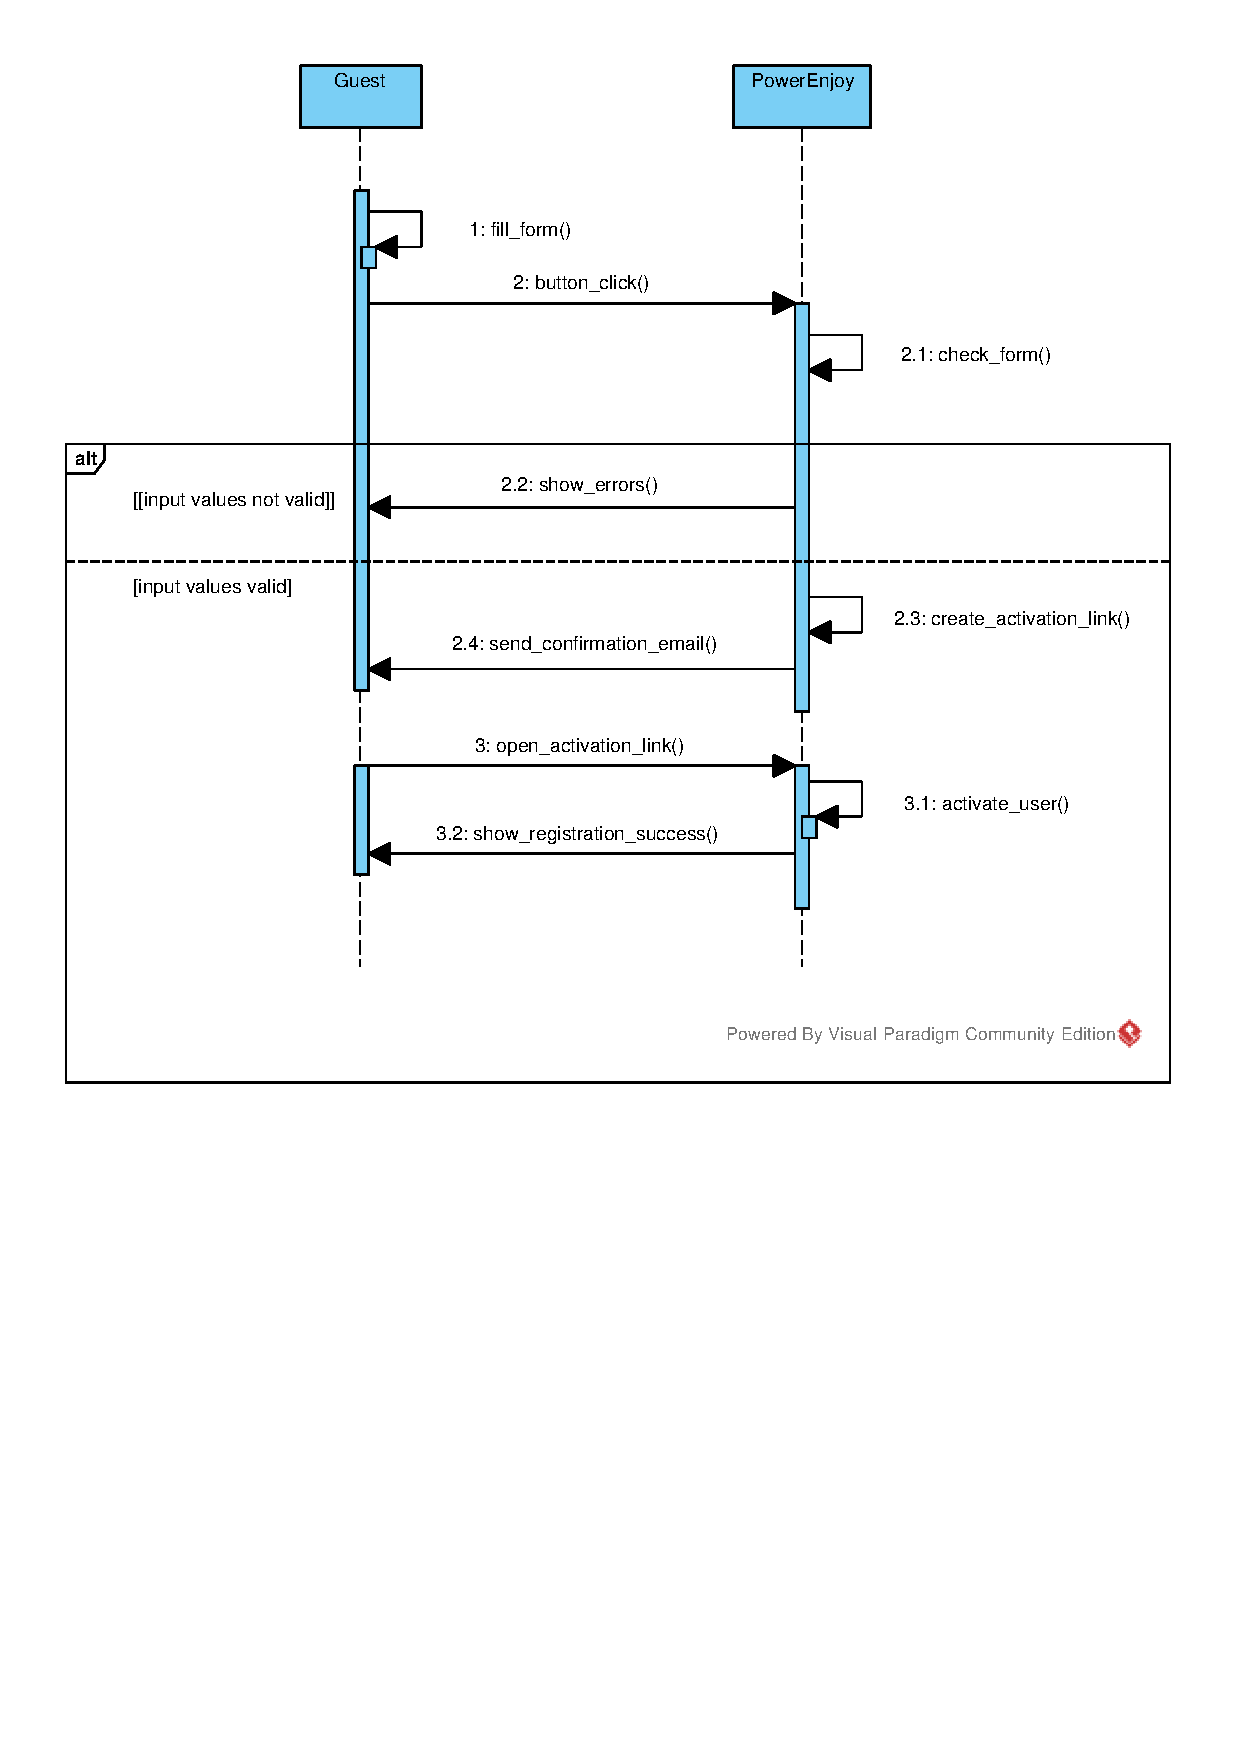
\includegraphics[width=\textwidth, keepaspectratio]{../images/diagram/sequence/registration.pdf}


\subsubsection{Car reservation through mobile or web application}
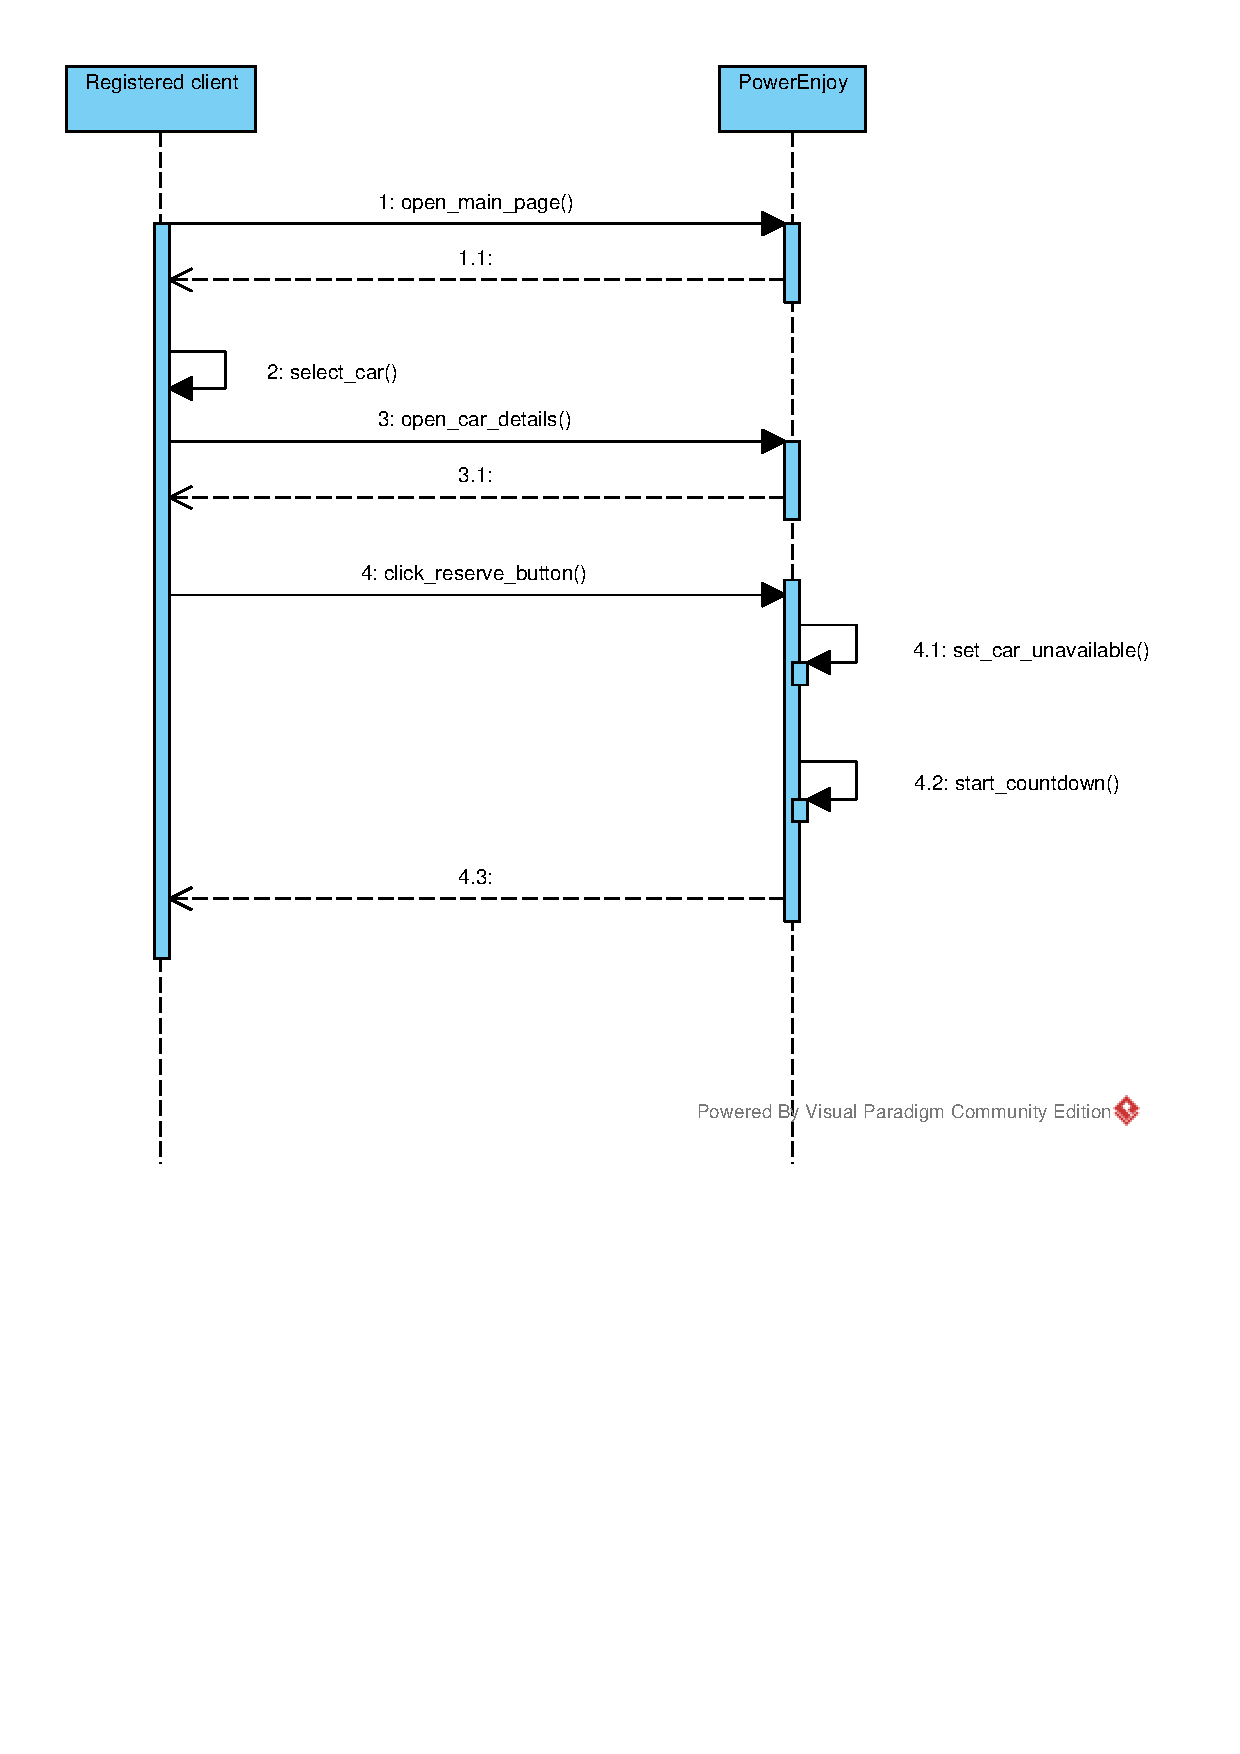
\includegraphics[width=\textwidth, keepaspectratio]{../images/diagram/sequence/reservation.pdf}


\subsubsection{Car reservation through SMS}
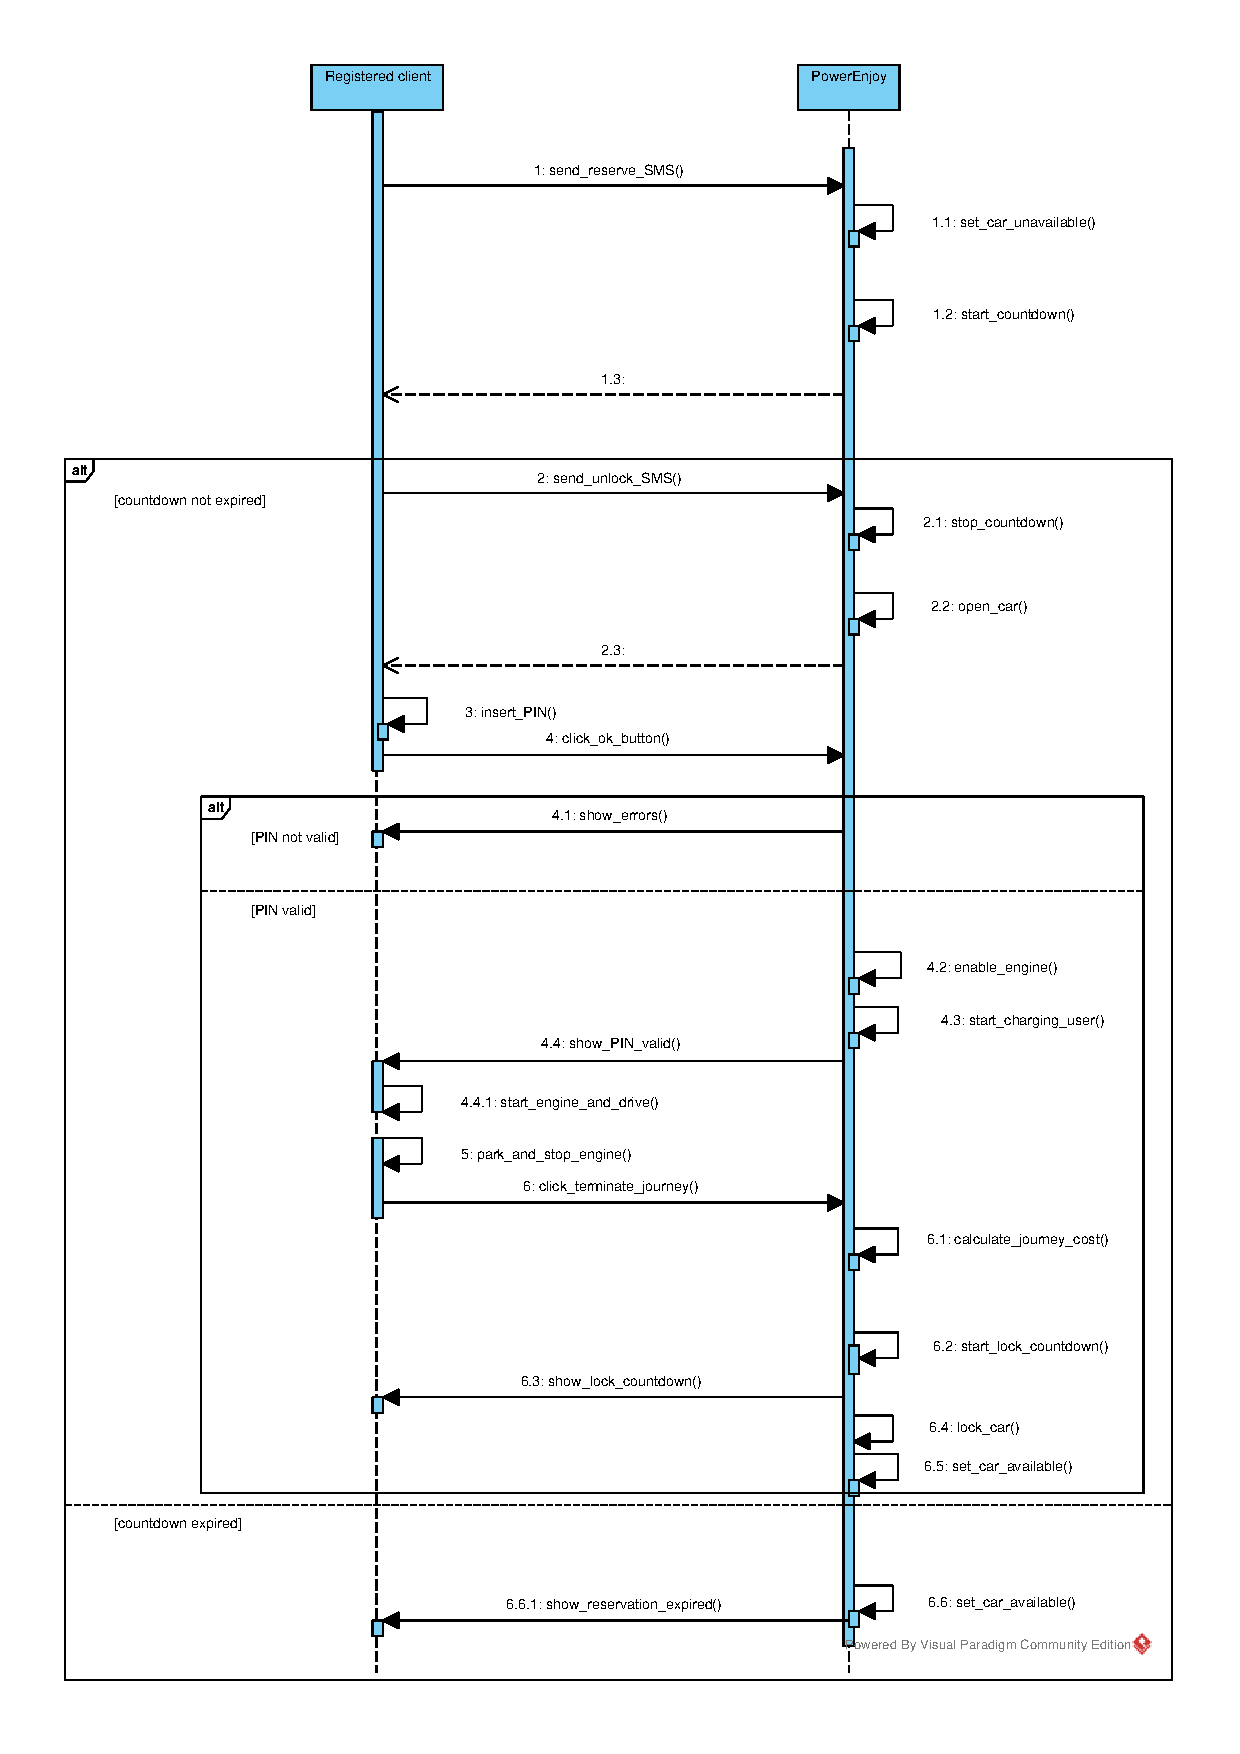
\includegraphics[width=\textwidth, keepaspectratio]{../images/diagram/sequence/sms_reservation.pdf}


\subsubsection{Cancel reservation}
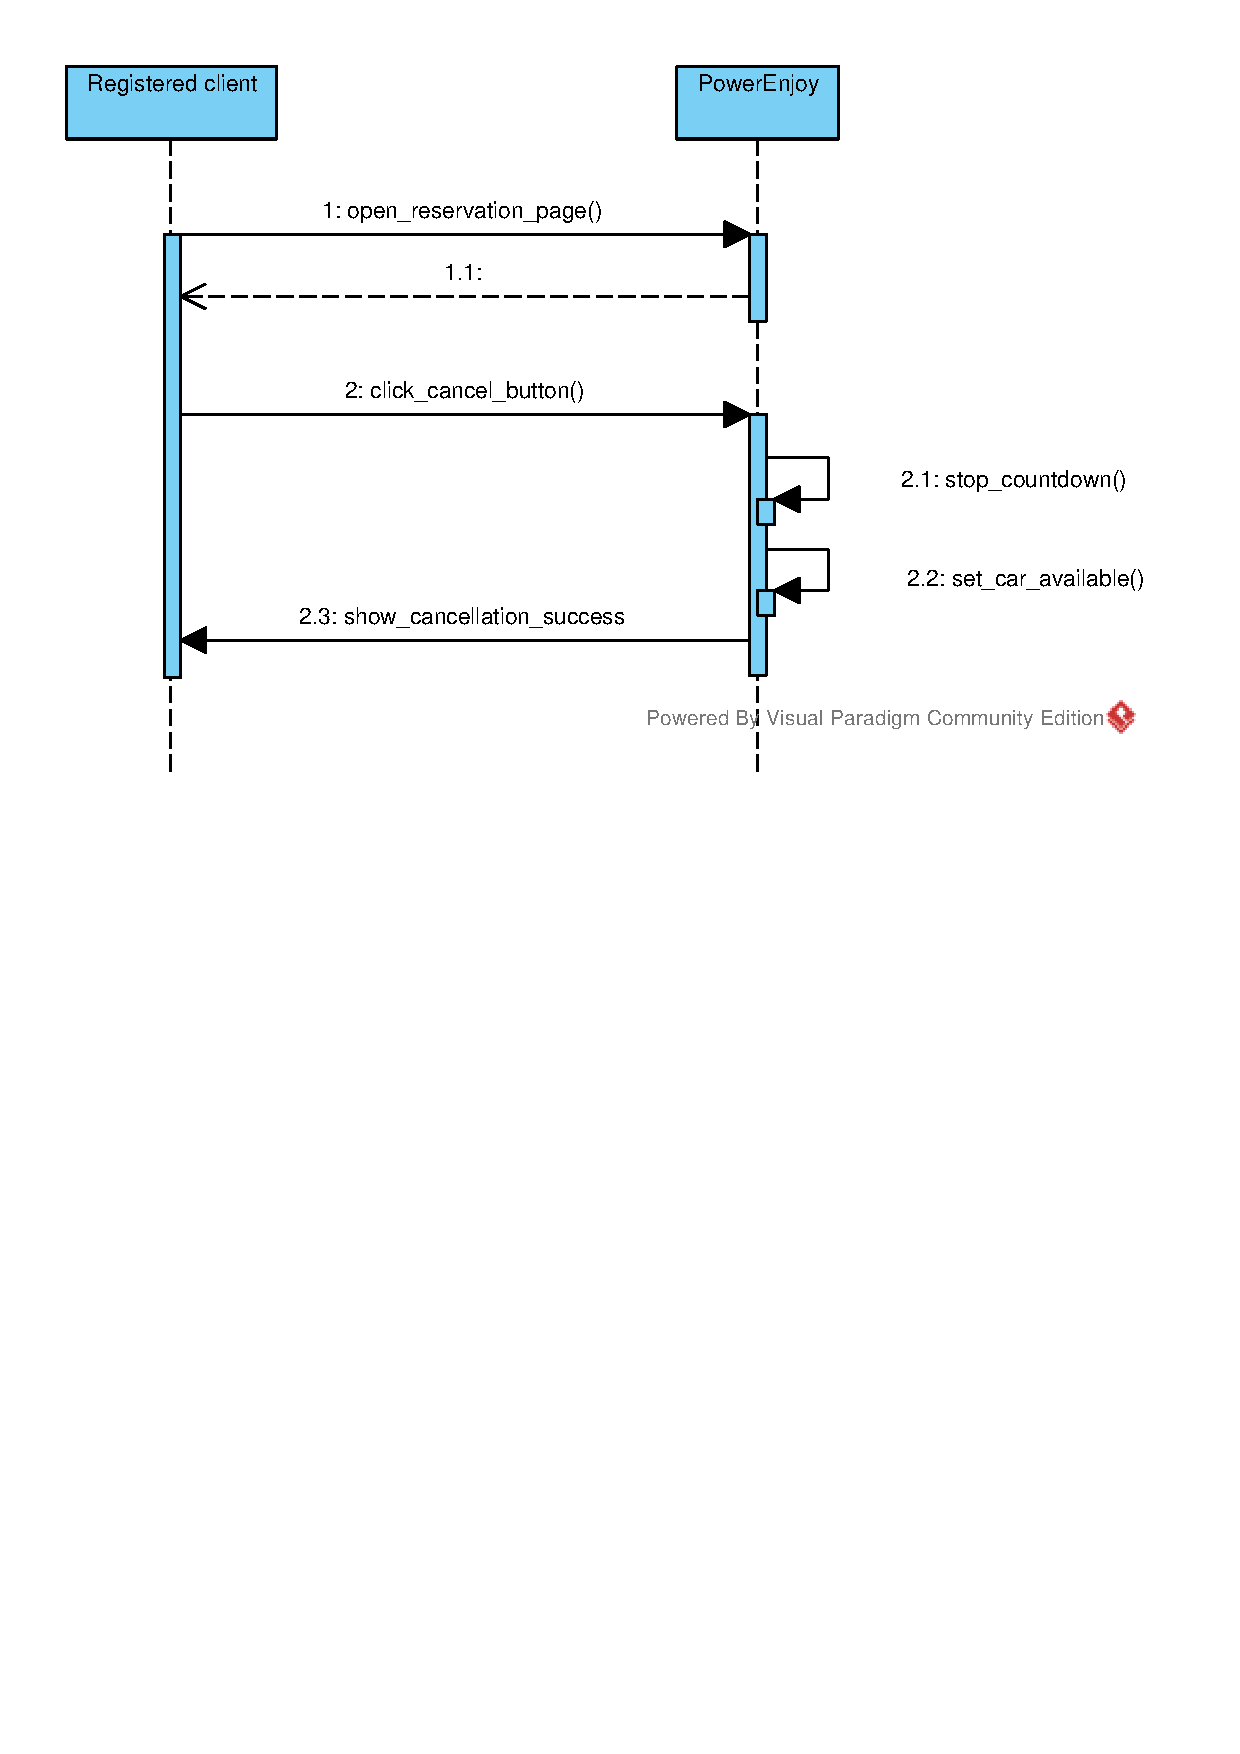
\includegraphics[width=\textwidth, keepaspectratio]{../images/diagram/sequence/cancel_reservation.pdf}


\subsubsection{Car usage}
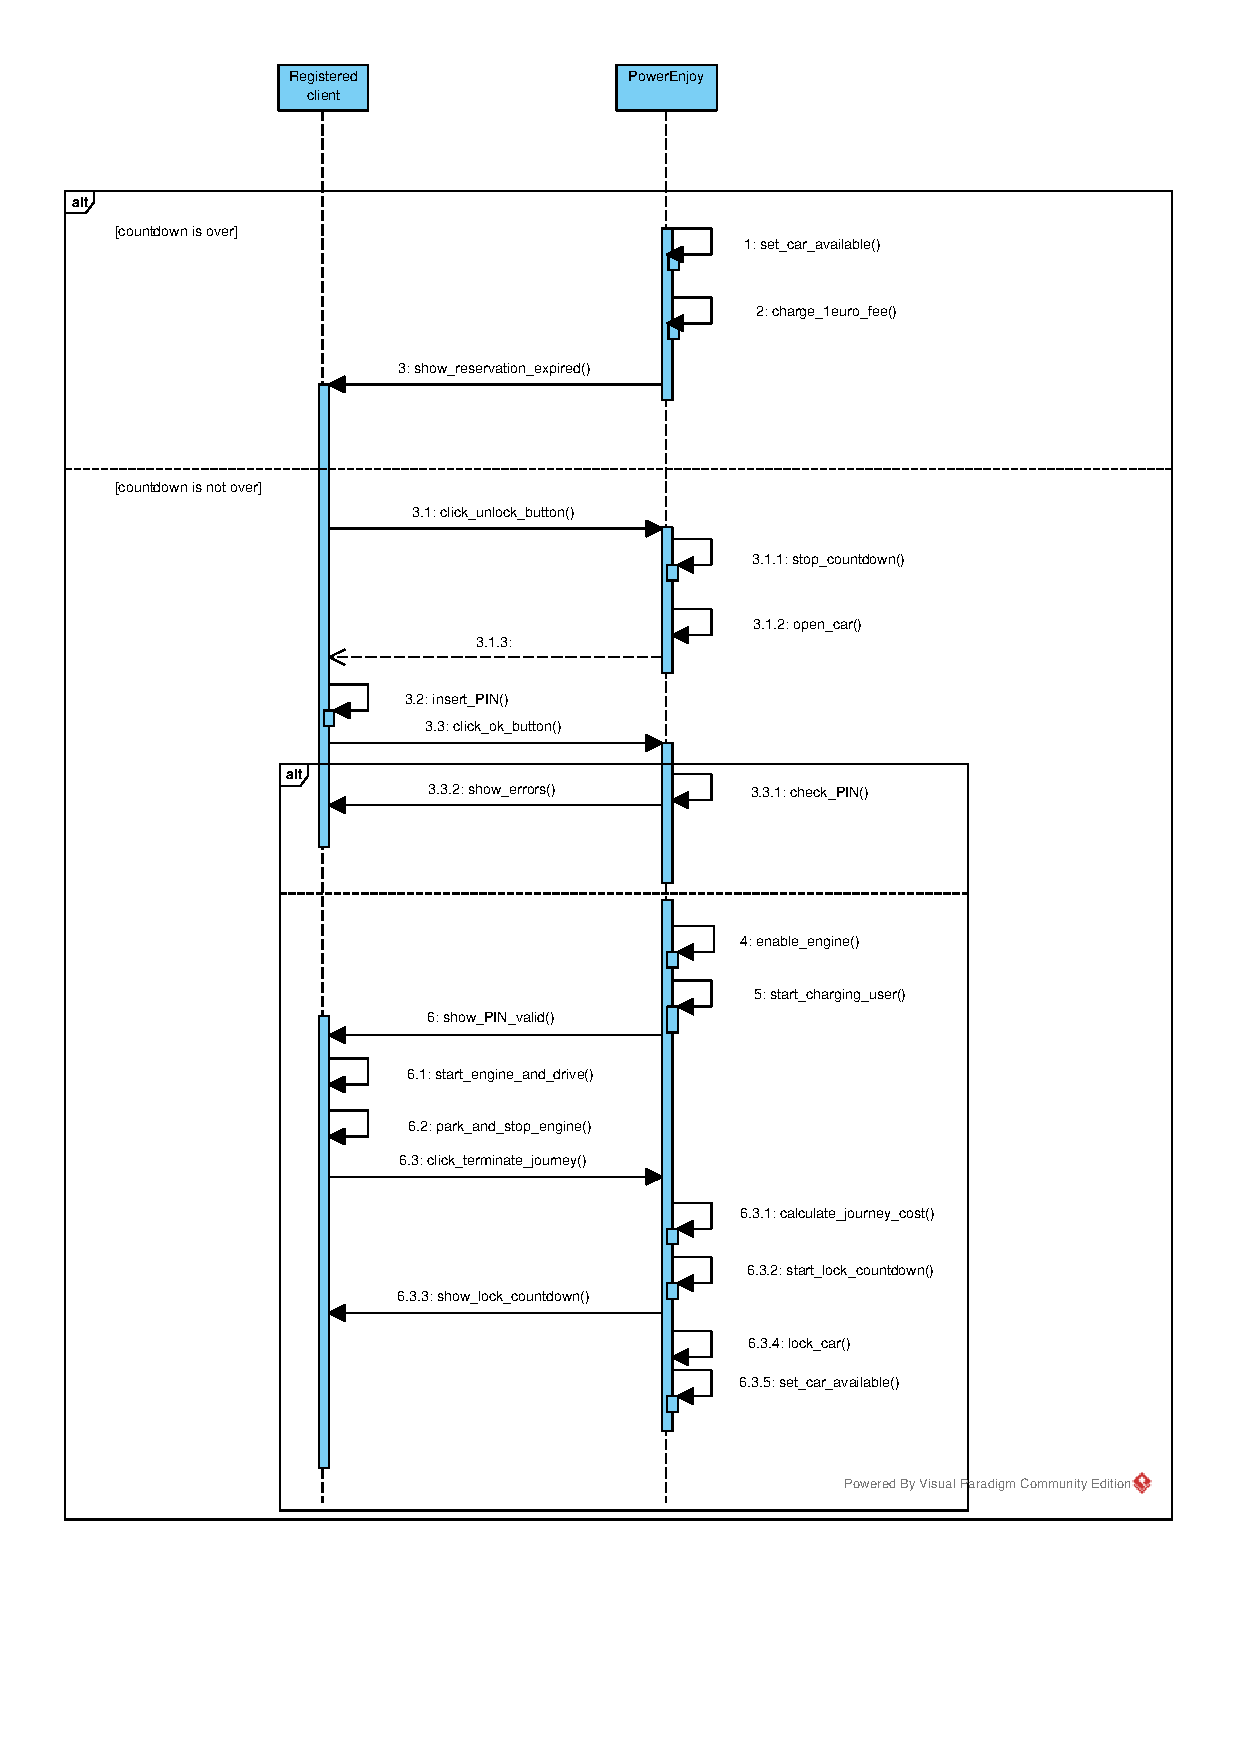
\includegraphics[width=\textwidth, keepaspectratio]{../images/diagram/sequence/car_usage.pdf}


\subsection{Class diagrams}

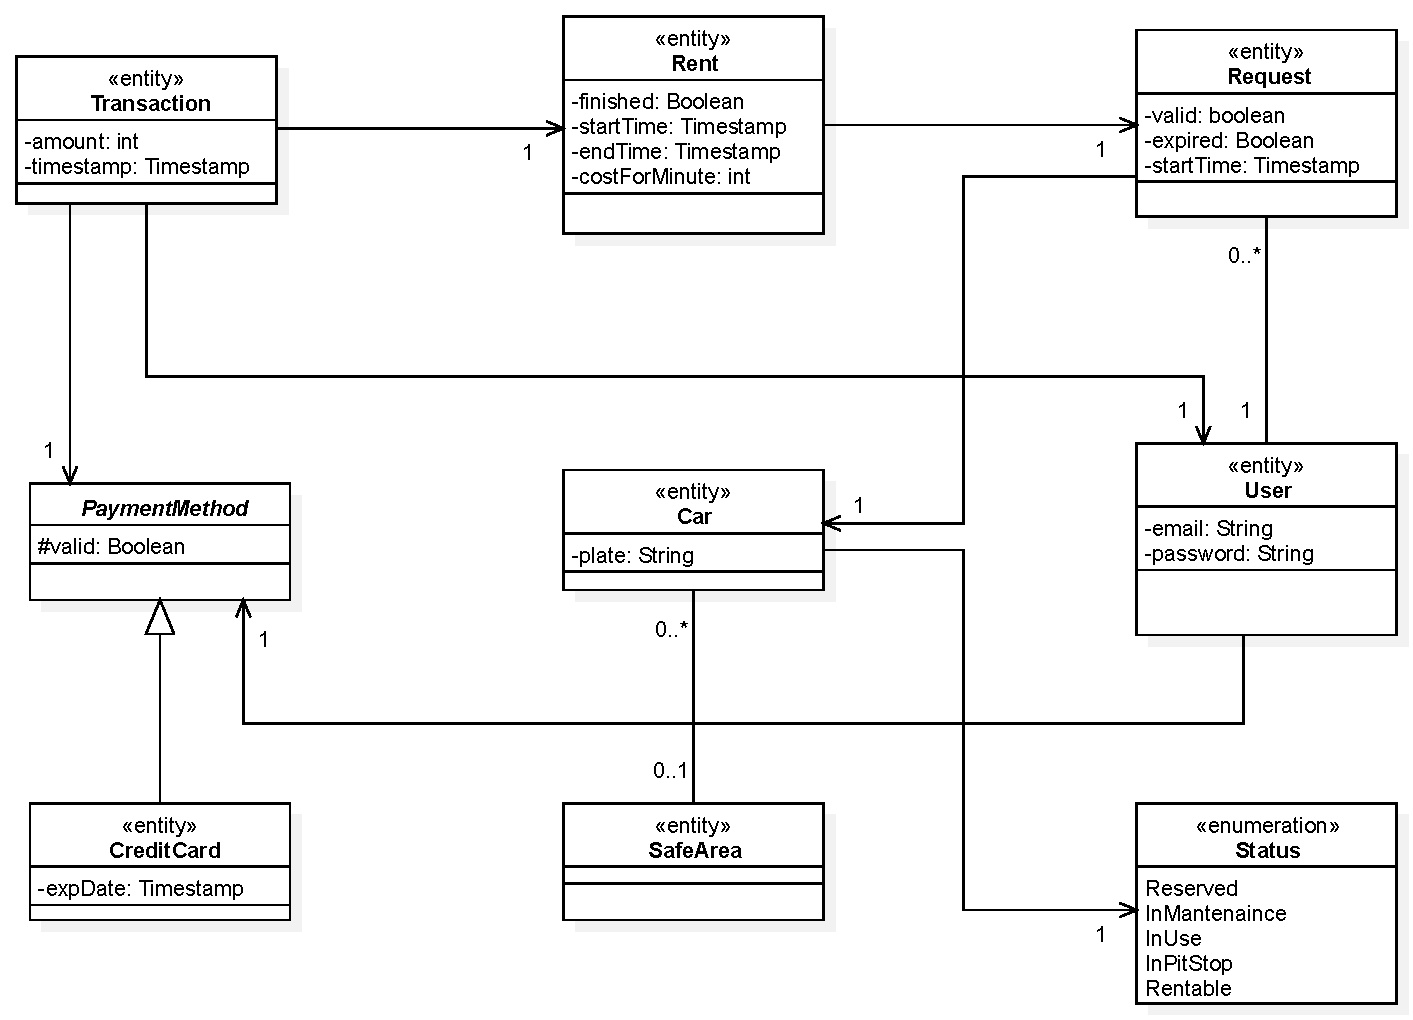
\includegraphics[width=\textwidth, keepaspectratio]{../images/diagram/class/class_diagram.pdf}

\subsection{State chart diagrams}
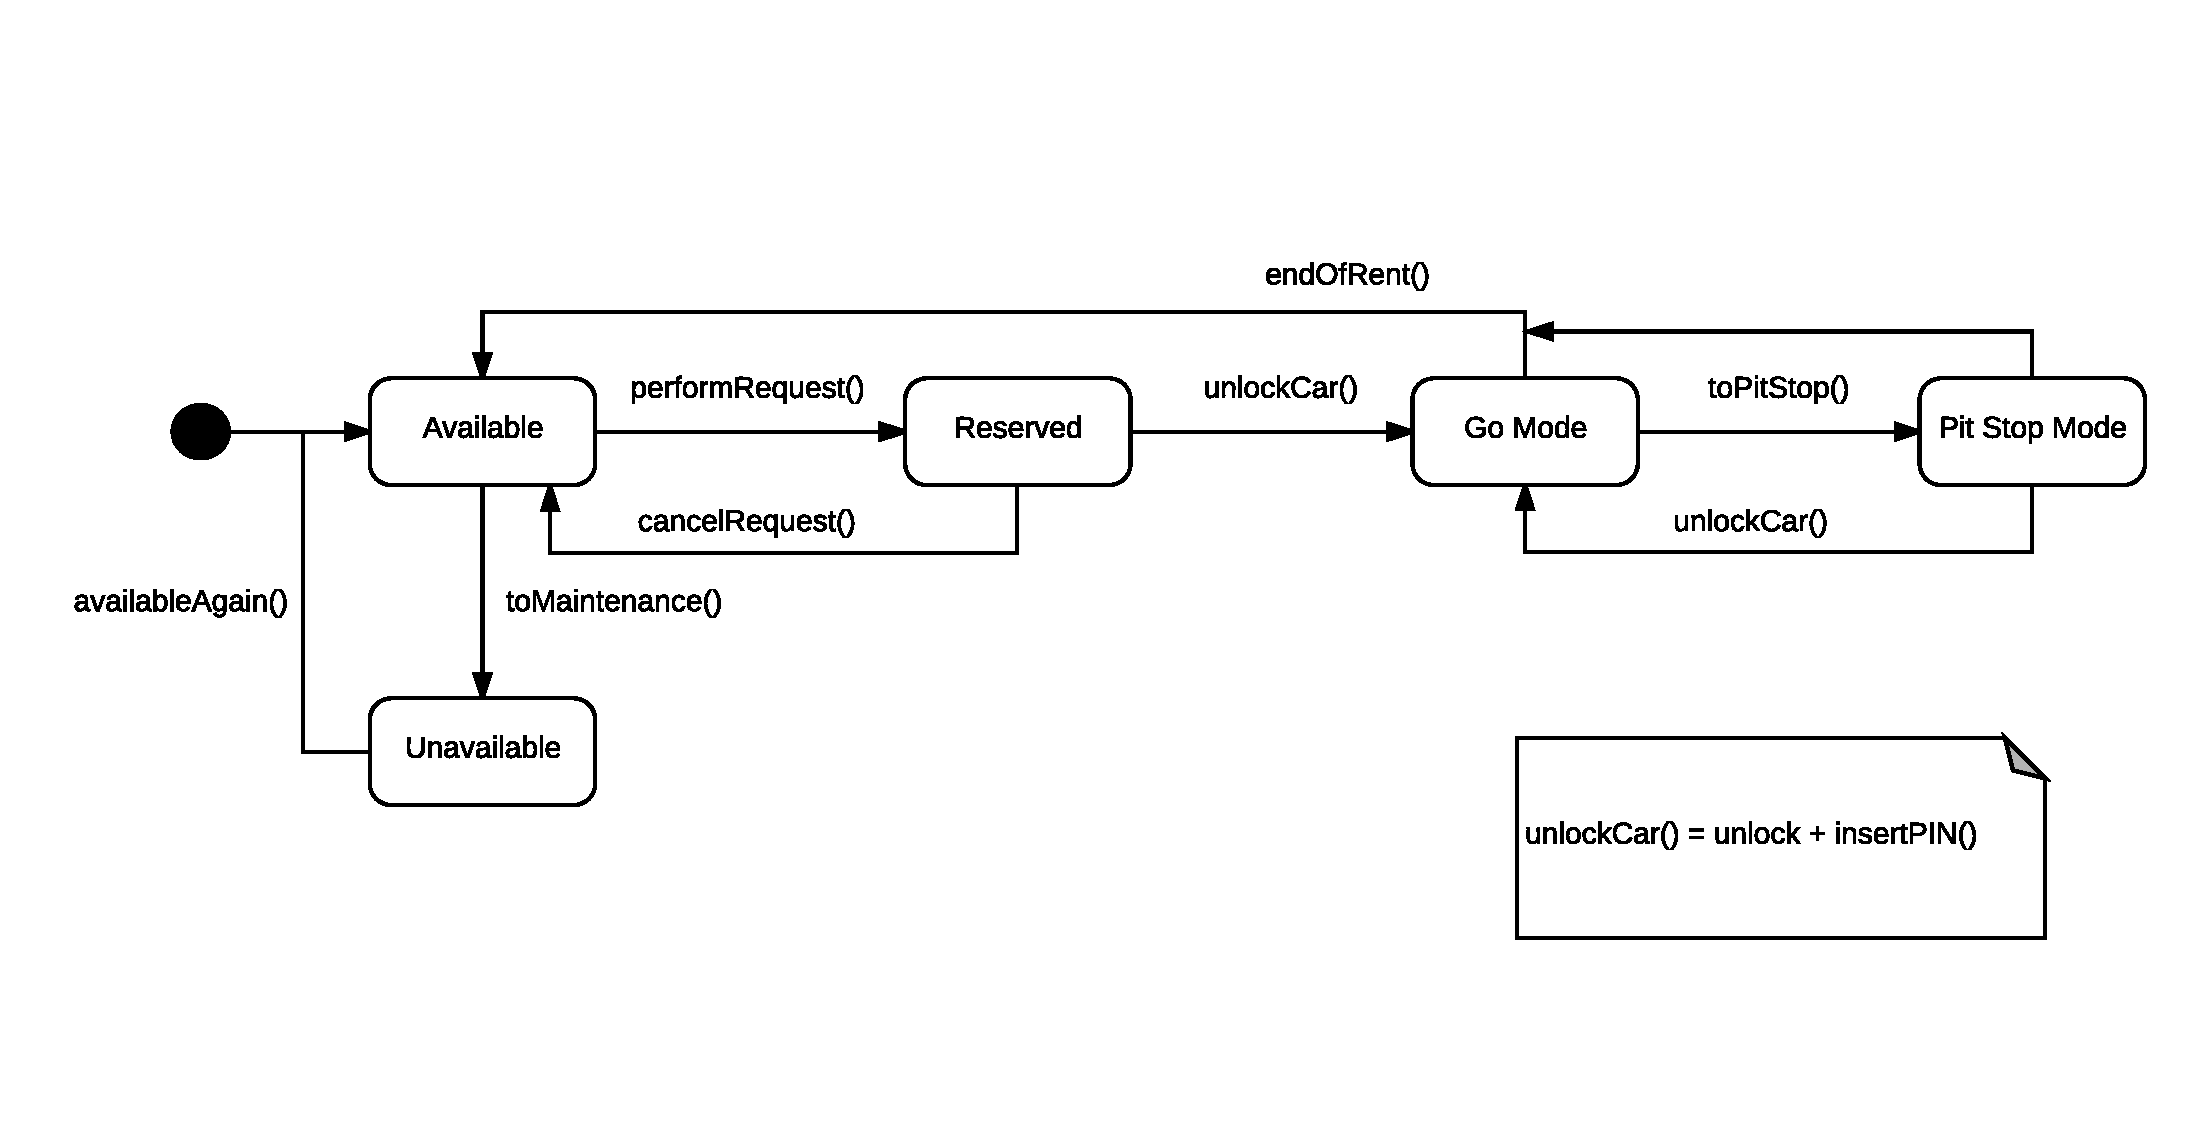
\includegraphics[width=\textwidth, keepaspectratio]{../images/diagram/state_chart/car_status.pdf}

\clearpage
\section{Non-functionals requirements}

\subsection{Performance requirements}
The system must guarantee that most of the operations have to be processed in less than 500 ms, in order to provide a real-time application.\\
If this target is achieved, the main boundary of the application is the user’s internet connection bandwidth.

\subsection{Design constraints}
The system architecture is organized following the MVC pattern, meaning that all the data are stored in the server side, all the business operations are done in the server side (M and C of the acronym) and the goal of the mobile and web apps is only to give an user friendly interface to interact with the system (V of the acronym).\\
The server side application is written in Javascript using Express.js as a web framework.\\
The android app is written in Java.\\
The iOs app is written in Swift.\\
The windows phone app is written in XAML and C\#.\\
The web application app is written in HTML5, CSS3 and Javascript using Riot.js as a UI library.

\subsection{Software system attributes}

\subsubsection{Availability}
The system must be accessible anytime, with a downtime ratio of 0.01 \%.\\
In order to achieve this goal the system uses Nginx as a proxy server.\\
This software manages more instances of the application server in order to have:
\begin{itemize}
\item load balancing, in order to let more users use the application concurrently
\item fault tolerance, in order to replace application server instances that incurred in fatal errors
\end{itemize}
\subsubsection{Maintanability}
The systems is highly maintainable thanks to the modular architecture that the MVC forces to use.\\
Each module is well documented, as well as the whole application, in order to help future developers to understand how it has been developed and organized.

\subsubsection{Portability}
The mobile application is developed for all the major mobile OSes.\\
In addition to this, the web application id design with a responsive layout in order to let users use it from any device with a modern browser.

\subsection{Security}
All the connection between clients’ app (mobile and web) and server are under secure websocket (wss).\\
This protocol is an analog of HTTPS, that uses SSL to avoid man-in-the-middle attack, encrypting all the data exchanged among the two parties.\\
Furthermore all the sensible data stored in our DB are encrypted, meaning that also the system administrator does not have access to those data.
